\chapter{Diseño del sistema}
\section{Diagrama de clases}
Se procede a representar el diagrama de clases indicando nombre de clases y tipos de relaciones.
Este diagrama de clases será representado en la figura \ref{fig:class_diagram}.

\begin{figure}[h!]
	\centering
	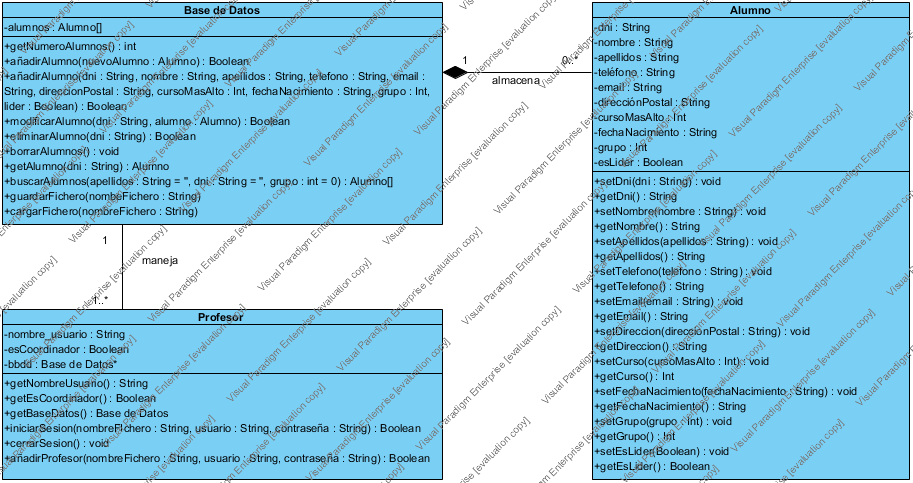
\includegraphics[width=1\textwidth]{../design/class_diagram}
	\caption{Diagrama de clases}
	\label{fig:class_diagram}
\end{figure}

\newpage
\section{Diagramas de secuencia}
El análisis de comportamiento se basará en los casos de uso previamente especificados y para
llevarlo a cabo se seguirá la metodología UML utilizando para ello la técnica de diagramas de
secuencias.

\subsection{Diagrama de secuencia. Añadir alumno}
\begin{figure}[h!]
	\centering
	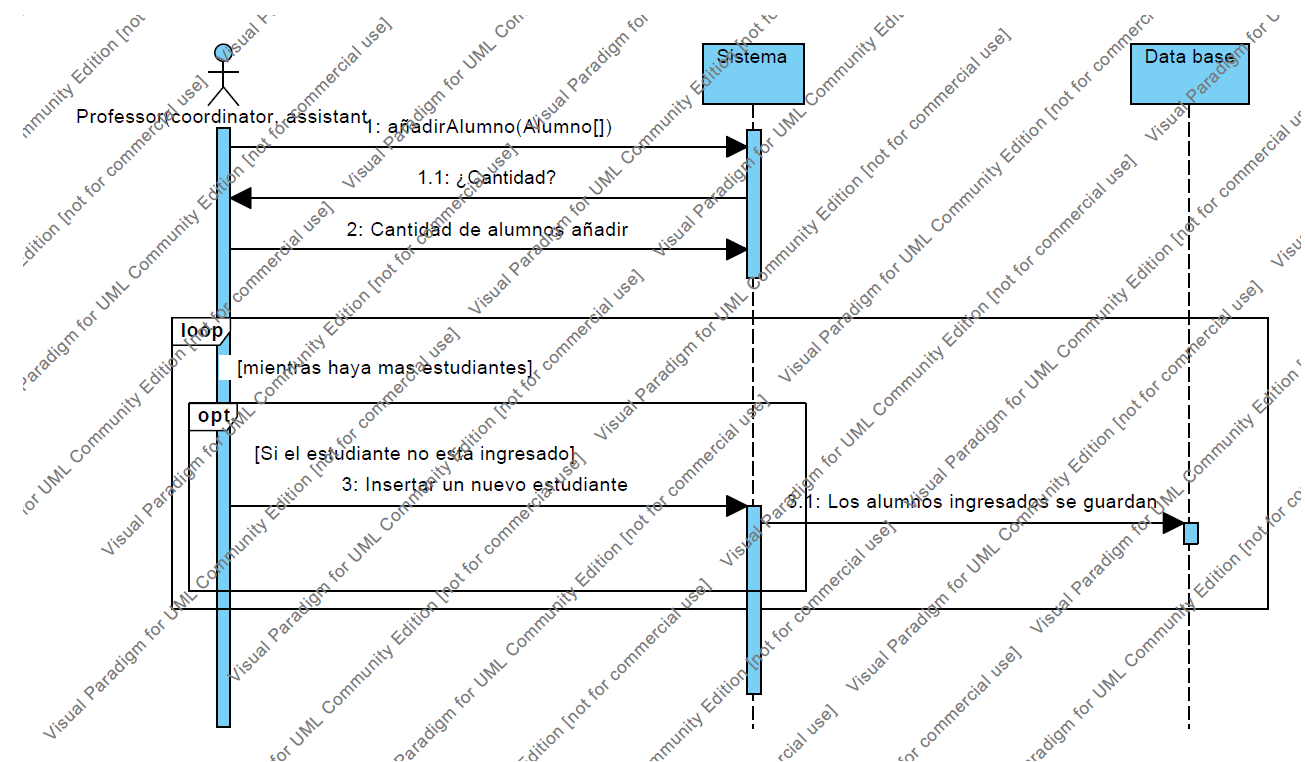
\includegraphics[width=1\textwidth]{../design/sd-1}
	\caption{Diagrama de secuencia del CU-1: Añadir alumno}
	\label{fig:sd001}
\end{figure}

\newpage
\subsection{Diagrama de secuencia. Modificar alumno}
\begin{figure}[h!]
	\centering
	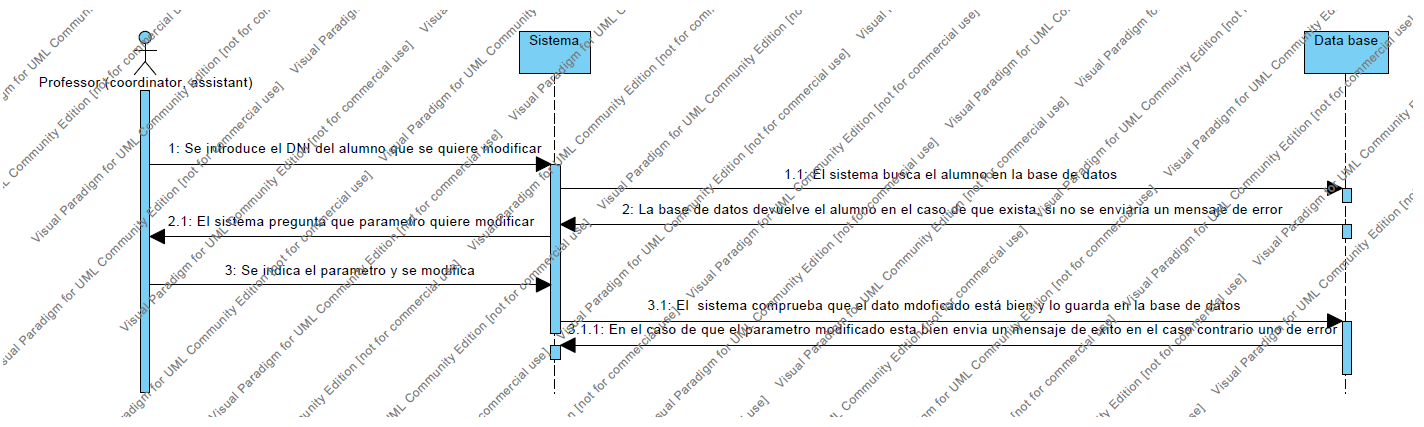
\includegraphics[width=1\textwidth]{../design/sd-2}
	\caption{Diagrama de secuencia del CU-2: Modificar alumno}
	\label{fig:sd002}
\end{figure}

\subsection{Diagrama de secuencia. Eliminar alumno}
\begin{figure}[h!]
	\centering
	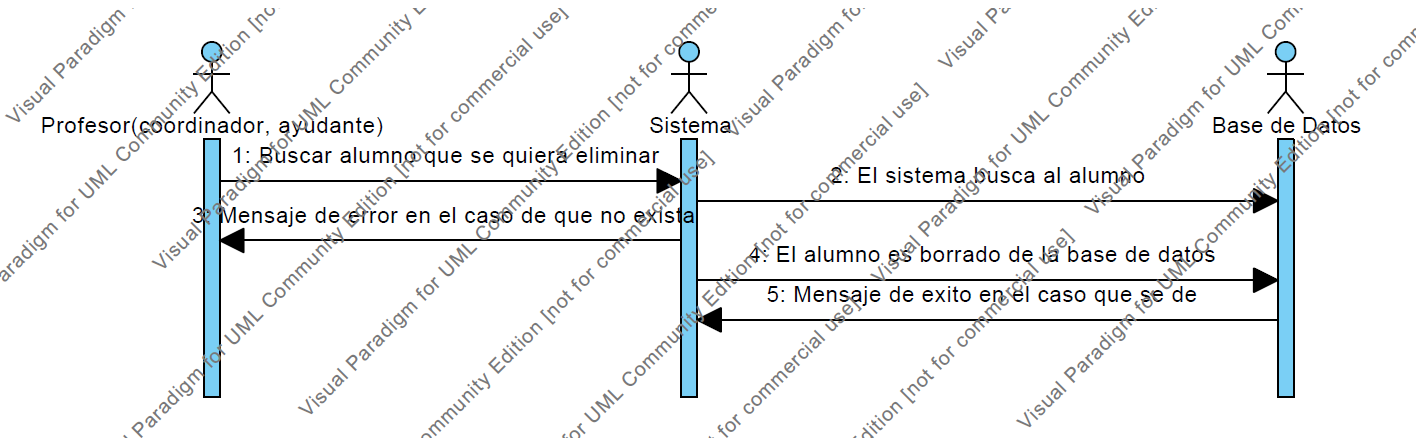
\includegraphics[width=1\textwidth]{../design/sd-3}
	\caption{Diagrama de secuencia del CU-3: Eliminar alumno}
	\label{fig:sd003}
\end{figure}

\newpage
\subsection{Diagrama de secuencia. Buscar alumnos}
\begin{figure}[h!]
	\centering
	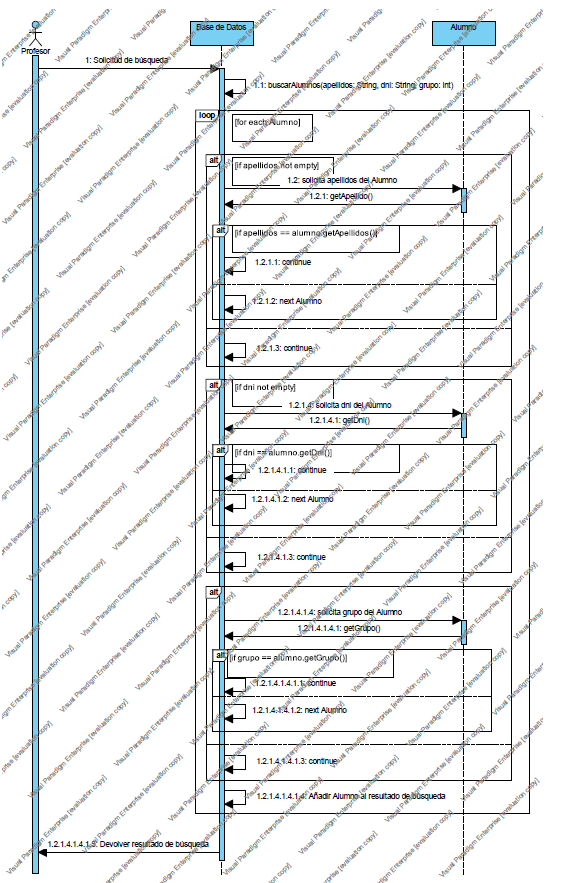
\includegraphics[width=0.75\textwidth]{../design/sd-4}
	\caption{Diagrama de secuencia del CU-4: Buscar alumnos}
	\label{fig:sd004}
\end{figure}

\newpage
\subsection{Diagrama de secuencia. Mostrar alumnos}
\begin{figure}[h!]
	\centering
	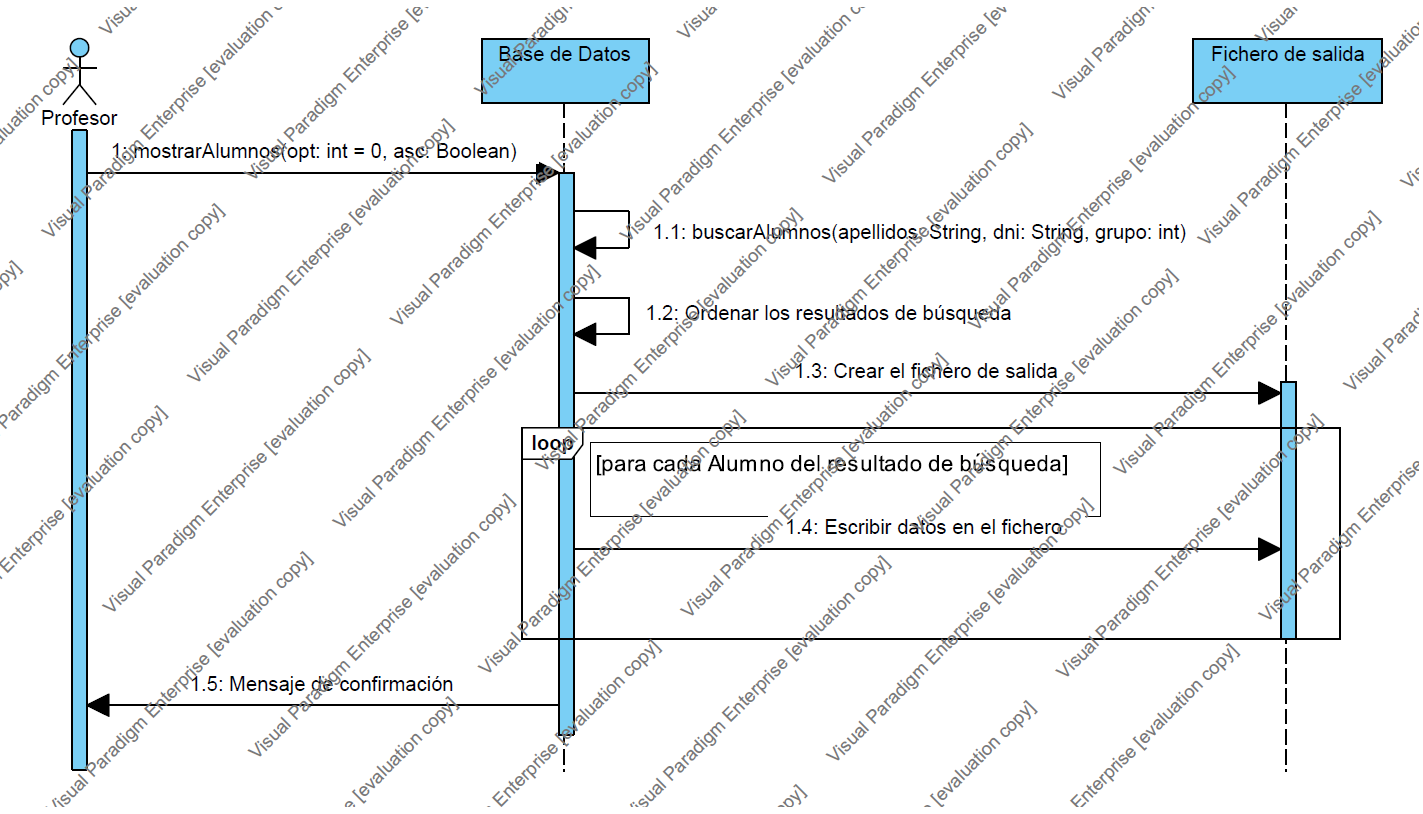
\includegraphics[width=1\textwidth]{../design/sd-5}
	\caption{Diagrama de secuencia del CU-5: Mostrar alumnos}
	\label{fig:sd005}
\end{figure}

\newpage
\subsection{Diagrama de secuencia. Guardar fichero}
\begin{figure}[h!]
	\centering
	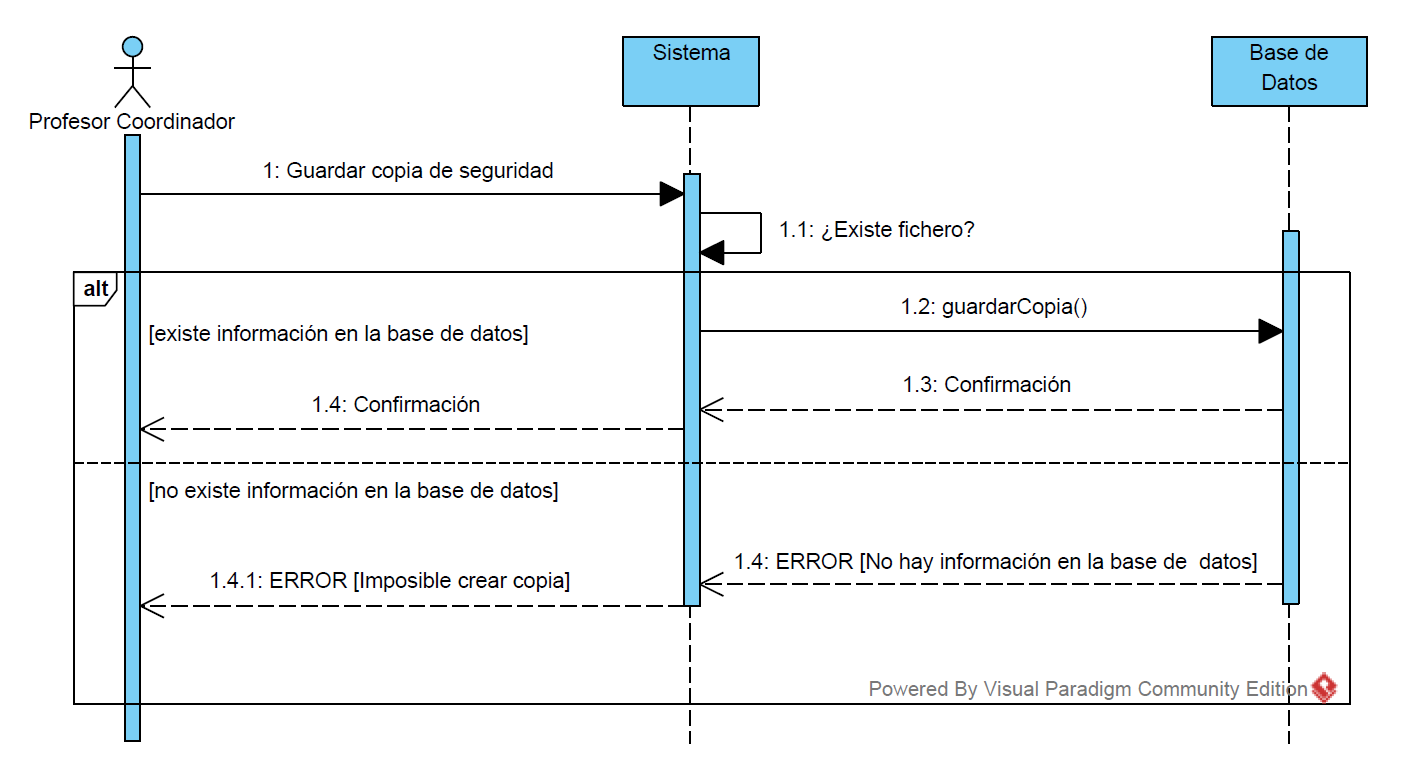
\includegraphics[width=0.9\textwidth]{../design/sd-6}
	\caption{Diagrama de secuencia del CU-6: Guardar fichero}
	\label{fig:sd006}
\end{figure}

\subsection{Diagrama de secuencia. Cargar fichero}
\begin{figure}[h!]
	\centering
	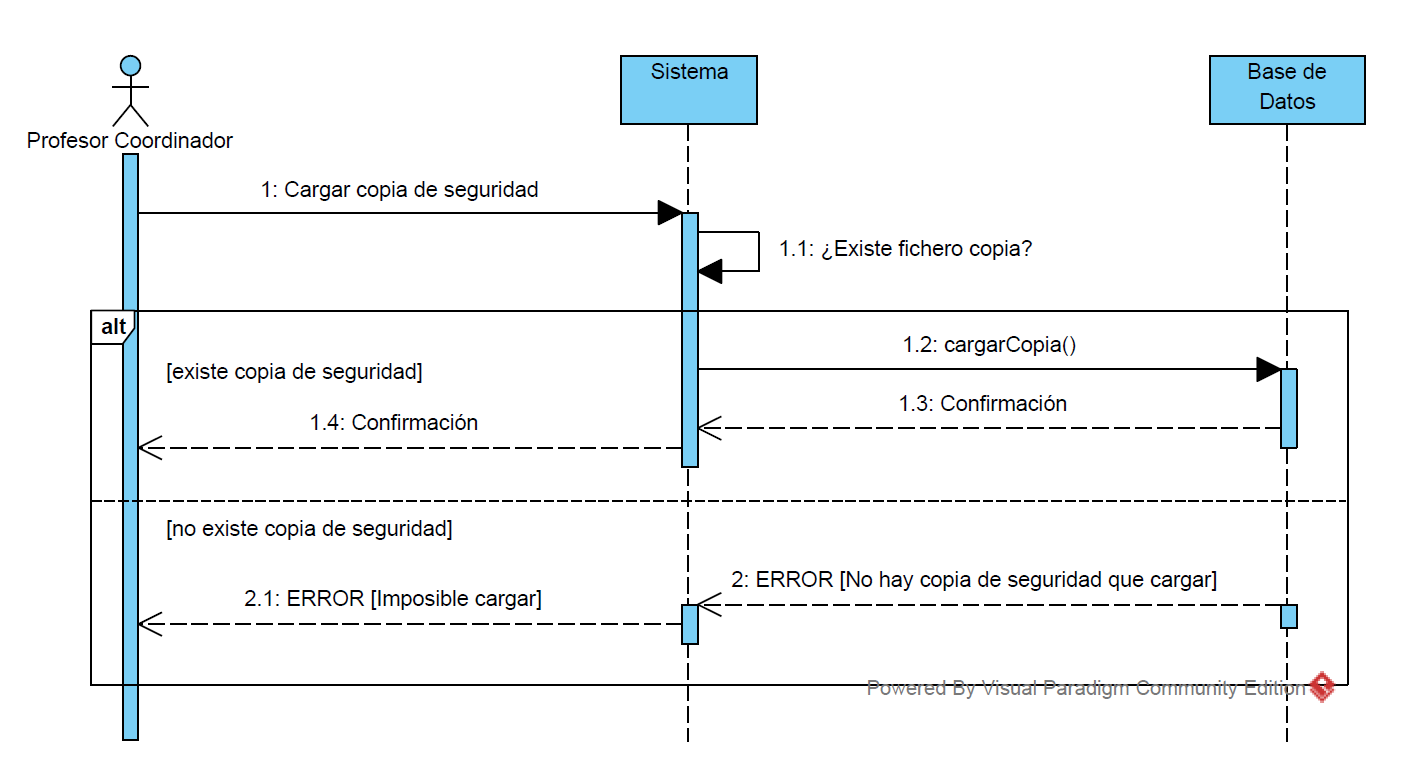
\includegraphics[width=0.9\textwidth]{../design/sd-7}
	\caption{Diagrama de secuencia del CU-7: Cargar fichero}
	\label{fig:sd007}
\end{figure}

\newpage
\subsection{Diagrama de secuencia. Identificar profesor}
\begin{figure}[h!]
	\centering
	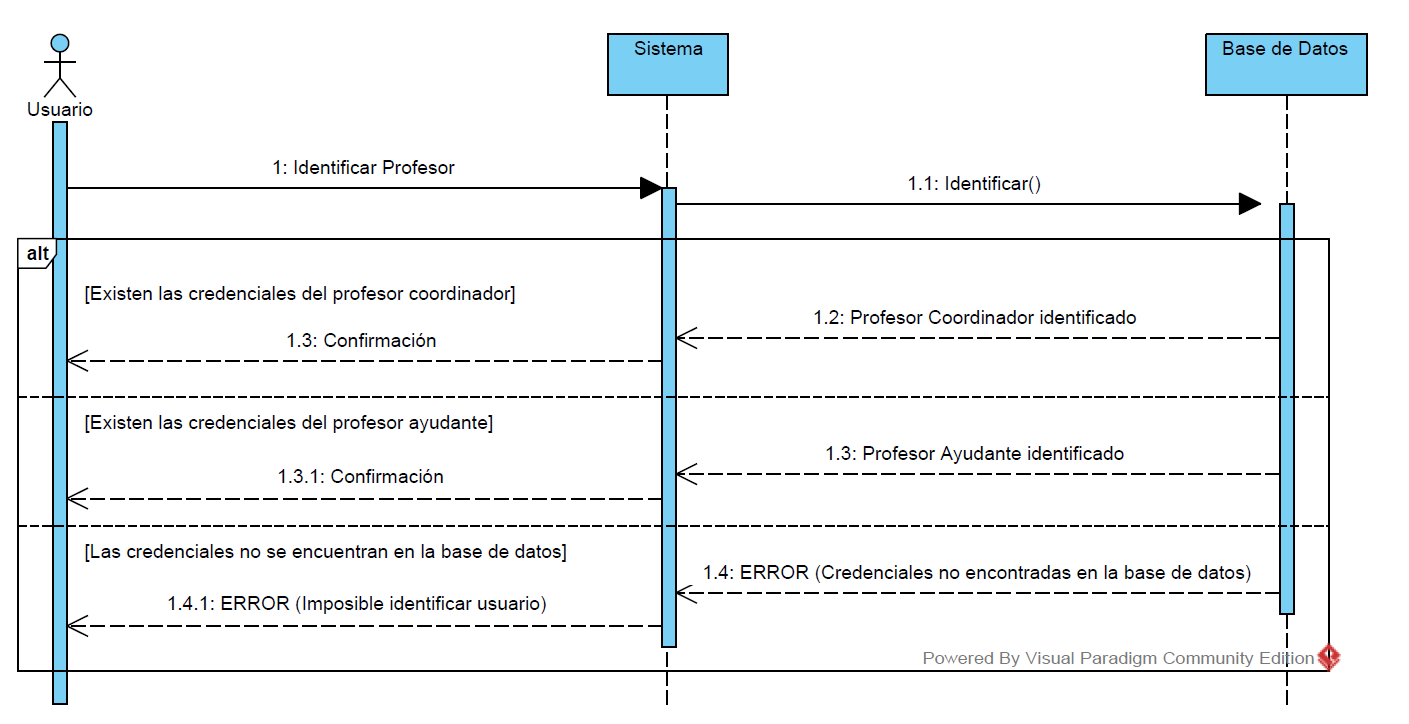
\includegraphics[width=1\textwidth]{../design/sd-8}
	\caption{Diagrama de secuencia del CU-8: Identificar profesor}
	\label{fig:sd008}
\end{figure}

\subsection{Diagrama de secuencia. Añadir profesor}
\begin{figure}[h!]
	\centering
	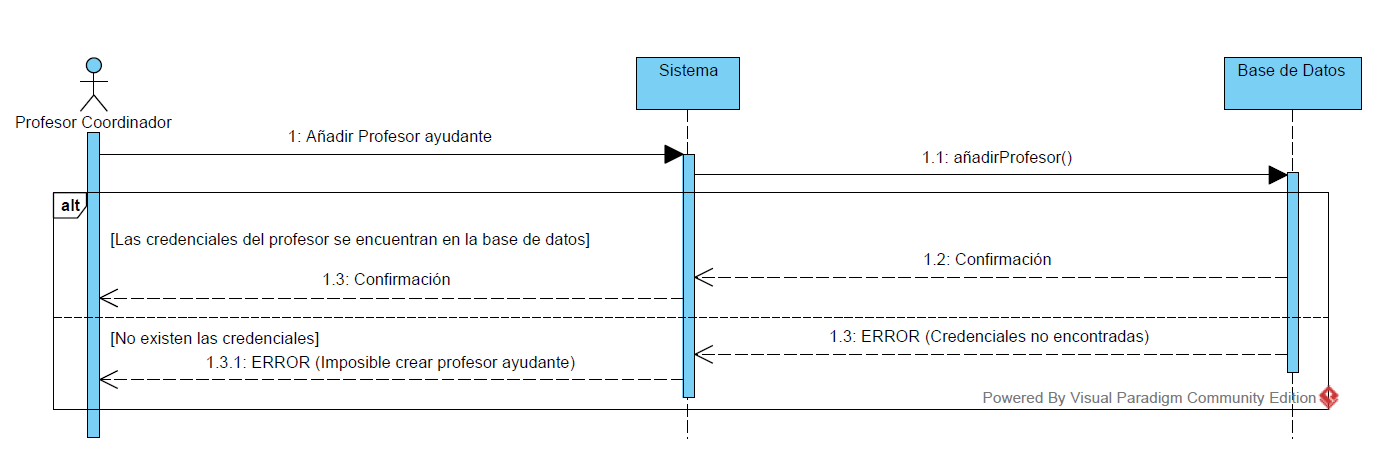
\includegraphics[width=1\textwidth]{../design/sd-9}
	\caption{Diagrama de secuencia del CU-9: Añadir profesor}
	\label{fig:sd009}
\end{figure}